\documentclass{article}
%% Language and font encodings
\usepackage[french]{babel}
\selectlanguage{french}
\usepackage[T1]{fontenc}

%% Sets page size and margins
\usepackage[a4paper,top=3cm,bottom=2cm,left=3cm,right=3cm,marginparwidth=1.75cm]{geometry}

%% Useful packages
\usepackage{amsmath}
\usepackage{graphicx}
\usepackage[colorinlistoftodos]{todonotes}
\usepackage[colorlinks=true, allcolors=blue] {hyperref}
\usepackage[utf8]{inputenc}
\title{Rapport du jeu akiba.}
\author{Marin Dorange Launey\\
		L1 info Gr 4B\\
        21601861}
        
\begin{document}
\maketitle

\begin{figure}[!h]
\centerline{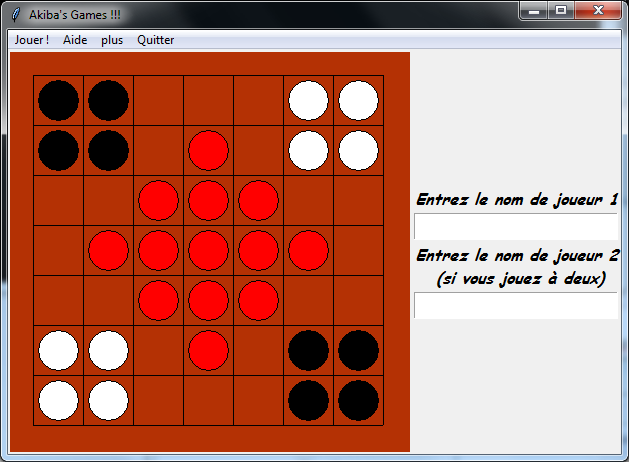
\includegraphics[width=0.6\textwidth]{images/Akiba.png}}
\vspace{1cm}
\caption{}
\end{figure}


\newpage{}
\tableofcontents{}

\newpage{}

\section{Introduction}

Le jeu d'akiba est un jeu de société creé en 1994 par Serge Cahu,il est aussi connu sous le nom de Traboulet ou encore Kuba.Il s'addresse aux enfants comme aux adultes.Malgré les rumeurs ce jeu est trés différents dans sa maniere de jouer par rapport au célèbre jeu de société Abalone. Toutes fois si vous souhaité acheté ce jeu de société en france vous ne pourrait pas car l'editeur de jeu Fun Connection ne le commercialise plus à cause de ces rumers. Nous avons donc,Dans le cadre du projet de methodologie 2016/2017 programmer ce jeu à l'aide de python et de quelque librairies telle que tkinter.

J'ai choisi ce jeu car il me rappeler le jeu d'abalone malgré ca grande différence,de plus ce jeu m'a plus facilement inspirée des idées que pour le latrncule.

\section{Aspect esthétique}
Pour l'esthétique, j'ai voulu choisir un style plutot rustique,neutre. Ce choix est du au fait que que le jeu inspire inspire la sagesse, la reflexion. Pour "faire" ce stylej'ai choisi que la grille pour jouer est un fond marron rappelant le bois et donc le théme proncipale.Ensuite même si l'on peut jouer sur les nuances, les couleurs des pions ont été definie selon les couleurs prédéfinie de tkinter (red,black,white). La police à été choisi pour continué sur le style rustique,neutre.Ainsi la police est noir, de type "comic sans ms". la taille varie selon que le texte soit un titre ou non.Enfin les titre sont en italic,gras et souligné.Pour finir la disposition du plateau, des menus et de l'affichage et, il me semble trés communes, en effet, le menus en haut, la partie jeu (ici le plateau) à gauche et l'affichage à droite se retrouv trés souvent dans les jeux flash,etc.

\section{Aspect technique}
\subsection{Fonctionalité de base}
\subsubsection{initialisation d'une partie en ligne de commande}
C'est une foctionnalité assez simple.On demande tout d'abord à ce que l'on saisissent le nom des joueurs. Ensuite on créez une grille remplie de boule, en effet on ne peut laisser des espaces vides,sans élément, dans une grille/liste.Ainsi les espace vides sont codé par des "boules" vides représenté par des "V", les boule noirs sont représenté par des "N", les boules blanches sont représenté par des "B" et enfin les boules rouges par des "R".Ensuite tant que le jeu n'est pas finie on demande au joueur qui doit jouer un mouvement et une position pour deplacer ses boules.
\newpage
\subsubsection{les mouvements}
 la fonctionnalité des mouvement regroupe 4 fonction,en effet, j'ai découpé cette fonctionalité en 4 fonction selon les 4 mouvement possible (Haut,Bas,Gauche,Droite). C'est fonction ont été pour moi des fonction dur à réalser.En effet le probléme qui se pose et que nous ne pouvons prédire la couleur des autres.

En effet, comme le montre l'exemple ci-dessous, ci nous voulons déplacer la boule blanche, on ne peut savoir si elle entrainera une boule noir ou rouge.Ainsi la premiére solution qui etait de mettre un rang plus loin la representation de la boule ne marche pas.Si on analyse la situation, on modifie notre support de travail,je m'explique,on met au rang n+1 de plateau ce que l'on voit au rang n de plateau or si l'on renouvelle une seconde fois l'operation,on met au rang n+2 du plateau ce que l'n voit au rang n+1 or precedemment le rang n+1 à déja changé de couleur.

\begin{figure}[!h]
\centerline{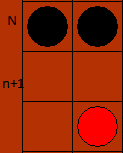
\includegraphics[width=0.2\textwidth]{images/fonctionalite_mouvement.png}}
\vspace{1cm}
\caption{}
\end{figure}

Ainsi sur ce morceau de plateau, on va mettre la boule noir du rang n au rang n+1, enfin on mettra au rang n une "boule" vide codé "V".Donc sur cette exemple tout ce passe bien. Ce mouvement effectué on se retrouve face à la boule rouge. C'est ici que, comme dit plus haut cela devient impossible d'effectuer un mouvement correcte.

\begin{figure}[!h]
\centerline{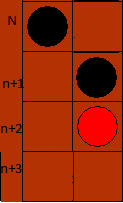
\includegraphics[width=0.2\textwidth]{images/fonctionalite_mouvement2.png}}
\vspace{1cm}
\caption{}
\end{figure}
Ici,si on déplace le pions noir au rang n+1,on mets au rang n+2 ce que l'on voit au rang n+1 ici une boule noir, puis comme la case n'était pas vide on continue le mouvement on mets au rang n+3 ce que l'on voit au rang n+2.Comme la case n+2 à etait changée juste avant ce n'est plus une boule rouge que l'on mettra mais une boule noir.
\newpage
J'ai donc eu comme idée de passé par une liste représentant la colonne ou la ligne de la grille sur laquelle on travaille,


\begin{figure}[!h]
\centerline{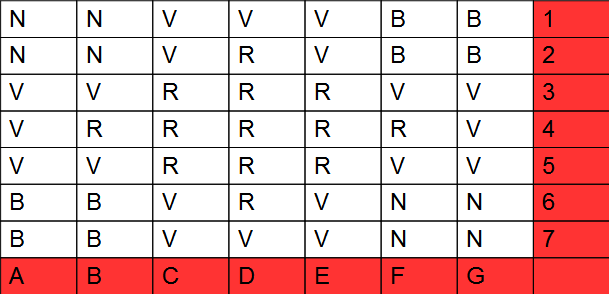
\includegraphics[width=0.6\textwidth]{images/schemas_plateau.png}}
\vspace{1cm}
\caption{}
\end{figure}

Prenons l'exemple d'un mouvement du pions noir noté 'N' en A2 vers la gauche, la representation de la liste sera donc:
\begin{figure}[!h]
\centerline{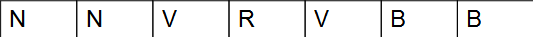
\includegraphics[width=0.6\textwidth]{images/ligne.png}}
\vspace{1cm}
\caption{}
\end{figure}


Par contre si on effectue un mouvement en A1 vers le bas, la representation de la liste sera alors:
\begin{figure}[!h]
\centerline{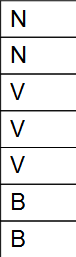
\includegraphics[width=0.1\textwidth]{images/colonne.png}}
\vspace{1cm}
\caption{}
\end{figure}

En faisant attention de copier la liste (d'ou la fonction copie) et non de faire une simple égalité entre ma liste et la liste représantant la grille(dans ce cas on ne copierait que l'addresse de la liste).Ainsi on mais au rang n+1 de la grille ce que l'on voit au rang n de la liste.
\newpage
\subsubsection{les test des mouvements}
Cette fonctionnalité de base à pour but d'obliger les joueur à respecter les régles. Ainsi je vais donc détailler les réges, la liste des contraintes.
\vspace{0.5cm}
\begin{itemize}
\item Une contrainte simple et prmiére on doit tout d'abord s'assurer que le pions que l'on veut pousser soit de la bonne couleur.

\item Une des régles et que le pions que l'on veut pousser ne doit avoir aucun pions dérriere lui, c'est à dire que l'on peut s'imaginer mettre sont pousse dérriere celui-ci sans risquer de toucher un autre pions.

\item On ne doit pas pouvoir pousser un de ses pions en dehors du jeu.

\item Enfin derniére régle, selon moi plus difficile à comprendre,on ne doit pas pouvoir annuler un coup précedemment joué par son adversaire. En effet si au tours d'avant l'adversaire à joué un coup qui à déplacé mes pions, je n'ai pas le droit de "remetre" ses pions.

\end{itemize}
\vspace{0.5cm}

Le points le plus difficile à été, pour moi, de vérifier que l'on ne sorte pas un de ses pions en dehors du jeu ou que l'on annule un coup précedemment joué par l'adversaire.
En effet pour les deux premiéres régle il suffit de regarder si la couleur du pions que l'in veut déplacer soit de la même couleur que celle du joueur qui doit jouer et que au rang n+1 ou n-1 se trouve une "boule" vide ou un bords du plateau.

\vspace{0.5cm}

Ensuite pour vérifier que l'on ne pousse pas un de ses pions en dehors du plateau, j'ai repris l'idée de la liste dans la fonctionalité mouvement.En effet je parcours,lit la liste et regarde si avant d'arriver à la fin de cette liste je tombe sur une "boule" vides et si j'arive à la fin, je regarde si la derniére boule est de la même couleurs que celle du joueur qui doit jouer, dans ce cas j'empêche le programme d'aller plus loin sinon dans tout les autres cas je le laisse effectuer l'action.

\vspace{0.5cm}

Enfin si l'on veut empecher un joueur d'anuler le mouvement réaliser par son adversaire il faut donne un peu de mémoires ou stocké les coordonnés, le mouvement effectuer ainsi que la liste représentant la ligne,colonne ou il a réalisé son coup.Le choix de variable à était un dictionnaire,ceci pour éviter d'avoir à retenir la position des éléments. Le probléme que j'ai rencontré au départ,est que je travallais sur la liste au coup n or je ne pouvais determiner si précédemment il y avais un espace ou si les boules des joueur était déja accolé. Pour résoudre cela j'ai ajouter la liste du joueur précédent comme indiqué plus haut, ainsi je regarde le coups n-1.

\subsubsection{la gestion des points}
Cette fonctionalité consiste à ajouter des points au joueur si celui-ci pousse une boule rouges ou une boules adverse en dehors du plateau et à verifier si un joueur n'à pas terminer la partie.Les points sont inscrits dans un dictionnaire ayant pour clé:
\begin{itemize}
\item le nom du joueur pour le nombre de boule adverse
\item le nom du joueur concaténé de la lettre "R" pour le nombre de boules rouges
\end{itemize}
\vspace{0.25cm}
Pour gagner il faut verifier une des deux condition suivante:
\begin{itemize}
\item Avoir pousser 7 boules rouges en dehors du jeu.
\item Avoir pousser toutes les boules adversesen dehors du jeu.
\end{itemize}
\vspace{0.5cm}
Pour la verification des boules pousser on s'inspire fortement de la facon dont on test si l'on pousse une de ses boules en dehors du plateau (cf: les test des mouvements). En effet on va parcourir la ligne ou colonne, plusieurs cas s'offre à nous:
\begin{itemize}
\item Si l'on rencontre une "boules" vides on renvoit notre variables inchangé.
\item Si l'on ne rencontre aucune boule vide et que la derniére boules est une boules adverse on renvoit notre variable ajouté de un points pour le nombre de boules adverse du joueur.
\item Enfin, si l'on ne rencontre aucune "boule" vide et que la derniére boule est une boules rouge on renvoit notre variable ajouté de un points pour le nombre de boules rouges du joueur.
\end{itemize}
Ensuite on vérifie que les scores maximale n'ont pas était atteinds pour l'un des deux joueur,Si c'est le cas on affiche alors un message pour l'avertir et on l'empeche de continuer de joué.


\subsection{Fonctionalité rajouter}
\subsubsection{Une interface graphique}
Il à était de mon avis qu'il était primordiale de mettre une interface.En effet ceux la rends,à mon gout plus facile l'utilisation du logiciel.
il faut cepandant réflechir à comment aborder certain point.En effet pour faire l'interface graphique il nous faut tout d'abord un plateau de jeu avec une grille. Ensuite il nous faut des boutons pour pouvoir activer les différentes options.De plus il nous faut une zone d'affichage pour pouvoir afficher les point,la couleur des pions des joueur ainsi que la couleur du pions qui doit jouer.Et pour finir il nous faut aussi une methode pour déplacer les pions.
l'interface proposé est donc celle-ci:

\begin{figure}[!h]
\centerline{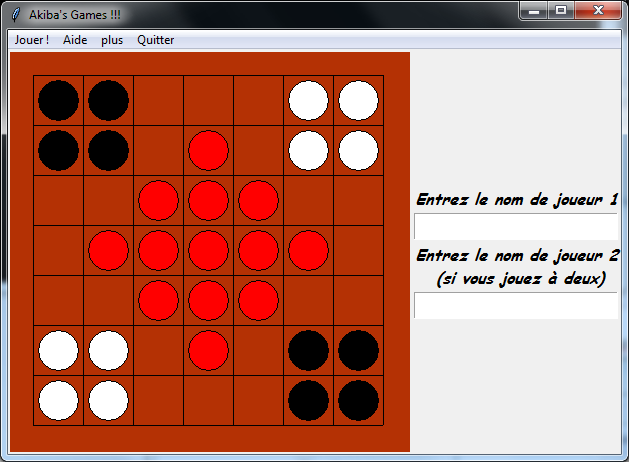
\includegraphics[width=0.6\textwidth]{images/Akiba.png}}
\vspace{1cm}
\caption{}
\end{figure}

Nous retrouvons donc en haut un menus tkinter permetant de déclenché différente action, Une zone d'affichage à droite ici avec deux zone de texte pour prendre les noms des joueur.Et enfin à gauche le plateau de jeu fait grace au canvas de la librairie tkinter.Il ne reste plus qu'a choisir la façon de déplacer les pions, J'ai choisi d'utiliser deux clic gauche de la souris représentant chacun un point pour à la fin obtenir un vecteur.
J'ai eu aussi à shouait d'éviter d'avoir plein de fonction pour récuperer les nom dans les zones de texte.C'est donc pour cela que ceux-ci sont présent depuis le lancement de l'application.

De plus j'ai rencontré des problémes quand à la mise en place de la methode de déplacement des pions.En effet ayant besoin de deux clics il faut verifier si l'on n'a pas déja cliqué juste avant et donc se souvenir du premier clic et remettre à zero lors du deuxiéme clic. Ainsi je suis donc passé par une variable globale nommé pos.Cette méthode étant trés pratique elle à néanmoins quelque lacunes,En effet si les clics ne sont pas précis la fonction interpréte mal ce que lui demande le joueur.

Enfin la translation des coordonnés du clic se fait par:
\vspace{0.25cm}
\\ 
x=floor((x1-25)/50)\\ 
y=floor((y1-25)/50)
\vspace{0.25cm}

Ou x1 et y1 représente les coordonnés x et y du clic de la souris.

\subsubsection{Une IA}
La seconde chose que je voulais rajouté était le fait que l'on puisse joué seul face à l'ordinateur.Pour cela il faut créer une sorte d'IA. Celle-ci doit être automatique c'est à dire que l'utilisateur ne doit pas avoir de boutton à appuyer, elle doit bien sur respecter les régles et surtout elle doit jouer de maniére aléatoire.

Pour l'automatiser j'ai donc fait appele à la fonction after de tkinter qui me permet d'appeler une fonction aprés un temps défini en miliseconds, Ainsi la fonction qui permet à l'IA de joit s'auto-appele aprés x seconde. Lorsque sont tour est arrivé, on parcours chaque case du plateau et à l'aide des fonction de test déja écrite on verifie pour les quatre mouvement possible (Haut,Bas,Gauche,Droite) si un coups est possible,Si c'est le cas on le rajoute à la liste des coups possible sous la forme [x,y,fonction] sinon on continue. Ensuite grace à la fonction choice du module random on choisit aléatoirement dans la liste des coups possible un coups.Ici apparait un petit probléme qui est que la fonction est de type chaine de caractére on fait donc appele à la fonction eval(arg1) qui execute la fonction qui porte le même nom que la chaine de caractére passez en argument si elle existe sinon elle renvoie une erreur.

\subsubsection{Un enregistrement,affichage des scores réalisé.}
Enfin la derniére chose que j'ai voulu faire, c'est d'enregistrer les scores de façon permanente,c'est à dire que même si on quitte l'application on puisse retrouver les scores que l'on à bien voulu enregistrer.Pour cela, tout d'abord lorsque l'utilisateur fini une partie une fenêtre,pop-up apparait lui indiquant qu'il à gagné et lui demandant si il veut enregistrer le score.Il lui suffit alors de cliquer sur oui ou non.Si l'utilisateur clique sur non rien ne se passera par contre
si l'utilisateur clique sur oui on enregistrera les scores qu'il vient de réaliser dans un fichier texte,on écrit les couples clés/valeurs du dictionnaire des points séparé par des /, ainsi si l'utilisateur quitte l'application il retrouvera toujours ses scores.Pour les relires il lui de demander à lire les scores ont lui demandera si il veut bien que le second joueur est etait l'IA ou non ainsi qu'un nom de joueur pour le retrouver dans le fichier.On lit alors le fichier et on ajoute à une liste chaque ligne, chaque scores enregistrer si il remplit les critaire demandés par l'utilisateur.

Pour l'affichage on ouvre une autre fenêtre à l'aide de la methode toplevel de tkinter cette methode permet que si on ferme la fenêtre principale celle-ci se ferme.Puis à l'aide de la méthode de placement grid de tkinter on se construit un tableaux (exemple ci-dessous) 

\begin{figure}[!h]
\centerline{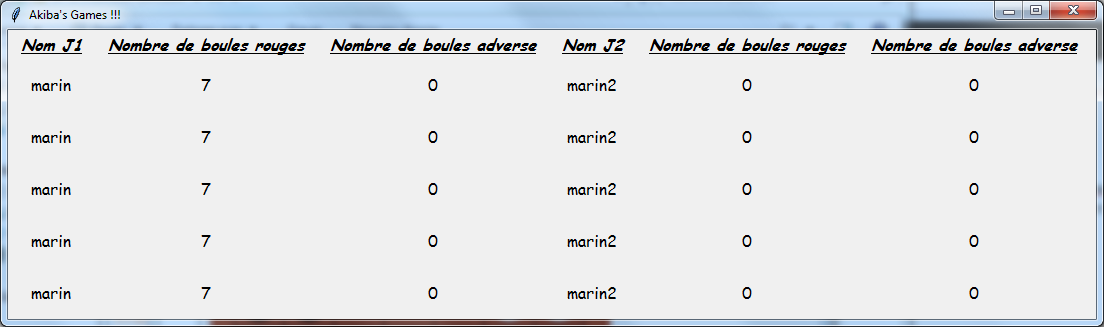
\includegraphics[width=0.9\textwidth]{images/Affichage_score.png}}
\vspace{1cm}
\caption{}
\end{figure}

Enfin si le joueur souhaite effacer tout les scores il disposent d'une option pour le faire.En effet on ouvre alors le fichier en mode ecriture ceux-ci à pour effet d'effacer le fichier.
\section{Suite voulue}
\subsection{Une IA plus inteligente}
L'IA programmé ici ne fait que tirer au sort bêtement un coup parmi tant d'autres, or j'aurai aimé pouvoir faire en sorte que l'IA choissise d'abord en fonction des points puis ensuite au hasards.
Les esquisse de programme pour implementer cette fonctionalité etait de passer la liste coups possible dans une fonction qui regarderait le maximum de points rapporté par un coups est qui ajouterait ces coups à une liste dans laquelle serai pioché un coups pour joué.
\newpage
\subsection{Une meilleur gestion des clic de la souris}
Comme amélioration voulue une meilleur gestion des clic est pour moi quelque chose de trés important.
En effet,prenons un exemple:
\begin{itemize}
\item X1=0
\item y1=0
\item x2=1
\item y2=6
\end{itemize}
D'aprés les coordonné donné plus haut notre bon sens nous pousserait à dire que, malgré un petits écart sur les x, le mouvement soit vers le bas,or pour mon programme il interpreterait ces point comme étant un coup vers la droite.
\subsection{Des bruitages et/ou animation}
Pour rajouter un peu de vie au jeu j'aurai aimé pouvoir rajouter des bruitages/animations.J'avais comme projet d'utilisé pygame pour écouter des sons en .wav,par contre, je n'est pour l'instant aucune piste à proposer pour ajouter des animation.

\section{Erreur et test de fonction représentative du programme.}
Tout ce qui sera dit sont les conclusions tiré des recherche de défaut des fonction important du programme éffectué dans le fichier "TestFonction.py".
\vspace{0.5cm}


\subsection{anti\_deplacement\_contraire}
La fonction est mise à mal tout d'abord lorsque l'on ne spécifie pas de "mode",en effet il n'y a aucun mode par défaut.
Ensuite la plus grosse erreur produite,est que si l'on spécifie en mode ecriture ("w") une liste qui n'a pas 7 élément mais moins. Or dans la fonction anti\_deplacement\_contraire on regarde au rang fixe 6 et on ne s'adapte pas à la longueur de la liste.
\subsection{B}
cette sous-section regroupe les fonction H,B,G,D
J'ai pu sur cette fonction trouver qu'une seule erreur.En effet celle-ci ne supporte pas que la liste, qui représente normalement la ligne ou colonne que l'on veut déplacer dans la grille,ne corresponde pas à la ligne ou colonne.

\subsection{test\_fin\_partie}
Aucune véritable erreur n'à était trouvé,seulement des incohérence.En effet il n'y a aucun test sur la cohérence des argument passé.Ainsi les deux joueur peuvent avoir le même nom voir un nom vide.Et,enfin, les noms qui doivent se retrouver dans les deux argument donner à la fonction peuvent être différents alors qu'il ne doivent pas pouvoir l'être.

\subsection{test\_Pions\_pousser}
On retrouve dans cette fonction les même erreur que dans la fonction test\_fin\_partie.Mais on peut rajouter le fait si le plateau n'est pas codé correctement (ex:on change la case majuscule minuscule) les valeurs retournés deviennent complétements incohérentes.

\subsection{traitement\_coordone}
Une unique erreur est formulé lorsque l'on spécifie un rang trop grand.

\subsection{test\_deplacement}
J'ai pu trouver une erreur,En effet on parcours la liste via une boucle for ... in range() or le range spécifier ne dépend pas de la liste passez en argument.Donc on obtient une erreur si on passe en argument une grille de 6*6 et non 7*7
\subsection{compte\_pions\_coul}
Comme dans la fonction test\_deplacementle parcour du plateau via une boucle for ... in range() pose problémme. On obtient donc on obtient une erreur si on passe en argument une grille de 6*6 et non 7*7
\subsection{search\_by\_name}
Ici je n'est pas réussi à trouver d'erreur cependant il y'a des incohérences à comprendre en effet on doit passer en second argument un booléen True ou False.Or on peut voir que une chaine de caractére non vide peut remplacer le booléen True et au contraire une chaine de caractére vide peur remplacer le booléen False.

\subsection{Grille\_Initiale}
Dans cette fonction deux erreur ont été trouvé. Tout d'abord si on passe en argument un tableaux plus petit que de taille 7*7 on obtien une erreur d'index car on ne tient pas compte de la taille du tableaux dans les boucle for.Ensuite si le tableaux est plus grand que 7*7 les ligne en plus ne seront pas modifié.

\section{conclusion}
Ce fut un projet fort intéressant.En effet malgré une apparence simpliste il c'est avéré difficile de construire certains point du jeu comme par exemple les fonctions de déplacement. Je suis néanmoins satisafait du résultat malgré des maladresse dans la façons de codé sur certains points.J'aurai aimé aller plus loin sur ce projet qui m'a véritablement prit à coeur de mener à terme.

























\end{document}